\section{Evaluation}
\label{sec:evaluation}

We evaluate \name through both experiments on real systems and numerical simulations. Results highlight:
\begin{itemize}
	\item \name reduces the average job completion time by a large fraction compared to existing methods and other baselines. \name retains significant improvements across various settings, even with relatively large estimation errors and overheads. 
	\item \name achieves comparable performance of \SRPT under a wide range of settings. Recall that \SRPT allows preemption at no cost and optimizes performance only with no fairness restriction. Informally, it can be considered as an unrealistic lower bound for the average job completion time.  
    \item \name provides fairness among users that is better than or comparable to existing fair allocation, and does not result in starvation for users with long jobs. Actually, \name provides the best progress for these users. 
	%\item \name retains significant improvements across various settings, even with relatively large estimation errors and overheads\todo{we need more figures to illustrate this point}.
\end{itemize}

\subsection{Setup}

\paragraph{Cluster} We setup Kubernetes with GPU support on a cluster of one master node, 8 CPU workers, and 4 GPU workers.
The master node does not execute any jobs. Instead, it coordinates the worker nodes and runs the job estimation tools. 
Each CPU worker is a \textit{xl170r} server from Cloudlab~\cite{cloudlab} with 20 virtual CPU cores and 64GB RAM.
Each GPU node is a \text{p2.xlarge} instance from Amazon EC2 with 1 K80 GPU, 4 CPU cores and 61GB RAM.
There are 4 users, which is increased in the simulations.

\paragraph{Workload} There are 4 users sharing the cluster. Each user has 10 popular Tensorflow jobs, e.g., Googlenet, Lenet, and Alexnet. The job configurations such as batch sizes and batch numbers are different, resulting in the speedup rates of using one GPU versus one CPU ranging from 1.8 to 10. 
For jobs on CPU, the number of threads is set at 19 to best utilize the virtual cores while leaving one core for other services on each node. 
We run a small sampling job for each real job to obtain the parameters for both CPU and GPU configurations, as we discussed in Section~\ref{sec:profiling}. 
The total overhead of sampling jobs is 3\% of the real jobs. We vary the settings in Section~\ref{sec:sensitivity} to evaluate the impacts. 
%Note that we cannot use 20 cores because there are other services are running on each node.
%\new{The fairness level is set at 0.5, meaning, we pick 2/4 of all users with the least fairness scores for scheduling overtime. }

\paragraph{Simulator} While experiments on real systems provide most realistic evaluations, it is costly to run in large scale over a long period. To fully evaluate \name, we implement a Java-based cluster simulator, which emulates the cluster with multiple resources, e.g., CPU, GPU, and memory. We validate the accuracy of the simulator by comparing its results to those from the real experiments over the cluster (Figure~\ref{fig:avgCmplt_exp}). 
%Jobs on the simulator can interchange between CPUs and GPUs.
%\todo{Add the setup information}
% For fair-cost comparison, we consider the CPU cores to GPU rate is 32.
There are 20 GPUs, 20 CPUs with 20 cores each, and 1280 GB RAM. %\todo{Tan, please check}.
%There are 10 users.

For numerical simulations, we use the workload trace from the Google cluster \cite{google-traces} to generate arrival times for Tensorflow jobs.
%The arrival times of our workload are the arrival times in the Google trace.
There are 10 users and over 1000 jobs for each user. %With more users, the improvements of \name is even larger. \todo{can we run a simulation with 20 users to validate this?}
By default, the fairness level $\alpha$ is set at $0.1$, meaning, we schedule jobs from the $1/10$ of all users who have the least progress whenever a node becomes available. The estimation errors are based on our experiments with sampling jobs whose sizes are 3\% of the corresponding real jobs and are around 10\% as we discussed in \S\ref{sec:profiling}. The impacts of the fairness level, estimation errors, and overheads are studied in \S\ref{sec:tradeoffs}, \S\ref{sec:estimation_err}, and \S\ref{sec:overhead}, respectively.
% \todo{Tan, please update the reference}.
% \new{
% The standard deviation of estimation errors is set 10\%.
% The total overhead of sampling jobs is 3\% of the real job.
% The fairness level, estimation errors, and overheads and  are studied and varied in \S\ref{sec:tradeoffs}, \S\ref{sec:estimation_err}, and \S\ref{sec:overhead}.
% }

\paragraph{Metrics} %We consider average job completion time, and fairness.
To evaluate the performance, we measure the average completion time of all jobs under \name and baseline algorithms.
%Users expect to have shorter average completion time.
We use standard deviation of progresses across users to evaluate fairness. %\todo{This is to be updated.}
For starvation, we focus on the progress of users with longer jobs. %we compare the top 1\% job waiting time.

\subsection{Baselines} 
\label{sec:baselines}
We compare \name to the following methods.

\emph{\ESRP} (equal share with shortest job first): \ESRP divides all resources equally among users statically. 
For a particular user, whenever a resource becomes available, \ESRP picks the job with the shortest processing time on this resource. For instance, if all jobs prefer GPUs, \ESRP first fills up all available GPUs with shortest jobs based on their processing time on GPU, and then fills available CPUs with the shortest jobs using CPU configurations. \ESRP needs the estimator to predict the processing time in different configurations.
%If a user does not use up her allocated resources, it is equally shared among users with queued jobs. 
% \new{
% To pick the job configuration, \ESRP first fills up all available GPUs configurations of waiting jobs and fills up available GPUs with the shortest ones.
% When GPU is full and there are waiting jobs, \ESRP fills available CPUs with the shortest ones using CPU configurations.
% If a user does not use up his allocated resources, it is equally shared by the other users.
% }
%\del{We first use SJF to schedule all jobs to GPU then use SJF to schedule remaining jobs to CPU.} %\zhenhua{This does not make sense. If you already put all jobs to GPU, then there is no jobs left.}
%\tanle{updated.}

\emph{\DRFFIFO} (online DRF with FCFS): %\del{If a job's completion time on CPU is shorter than that on GPU, it is placed on CPU, and vice versa. }
%\todo{Xiao, how is DRF calculated? Does it need profiling to know the demand, or you simply run FIFO and pick the user with the lowest progress?}
Whenever a resource becomes available, \DRFFIFO schedules the first job of the user with the slowest progress.  
Therefore, jobs are processed in a First-Come-First-Served manner within every user. 
For job configuration, we assume users have some preference. If all jobs prefer GPUs, \DRFFIFO always picks the GPU configuration. 
\DRFFIFO does not need the estimator to pick the configuration, and users' progress can be updated whenever a job is completed. 
%     Each job only has a single configuration that is chosen by users.
%     As DRFFIFO does not have 
% 	Hence, a job only has a single configuration and DRF does not need to handle the interchangeability.
%\tanle{updated.}



% Since \DRFFIFO schedules jobs based on their arrivals, it does not need the estimator.
% Like existing systems like Kubernetes \cite{kubernetes}, every job is predefined with a single configuration.
% In practice, users prefer to run their jobs on GPUs because GPUs are often more powerful than CPUs.
% So, we assume all jobs are configured to run on only GPUs with a large memory request (maximum memory of a node).
% Online DRF is used to allocate the single-configuration jobs with 2 resources (GPU and memory) like \cite{drf}.
%\zhenhua{I think we can add another baseline of just FIFO} 

	
\emph{\DRFSJF} (DRF with shortest job first): \DRFSJF is similar to \DRFFIFO, but within each user, jobs are scheduled in a shortest-job-first manner. Therefore, the estimator is needed. Each user relies on the estimation to pick whether CPU or GPU for each job configuration. 


% When a GPU (or CPU) becomes available, \DRFSJF picks the user with the lowest progress and schedule her job with the smallest processing time on GPU (or CPU, respectively).
% We consider another baseline using DRF that uses SJF to schedule the jobs. \todo{Xiao, again, how is DRF calculated?} \tanle{updated.}
% \new{
% Since \DRFSJF schedules jobs within a user, it need the estimator to estimate the completion times of jobs on both CPU and GPU configurations.
% \DRFSJF chooses the most effective configuration based on the estimated completion times.
% Online DRF is used to allocate the single-configuration jobs with 2 resources (GPU and memory) like \cite{drf}.
% }
% \zhenhua{From the results, CPU utilization of \DRFSJF is low. Does this mean when a CPU is available, \DRFSJF does not always schedule jobs on that? If so, we need to adjust the description accordingly.}

\emph{\DRFExt}: \DRFExt uses some average speedup rate to convert GPU resources to the corresponding CPU ones, e.g., if the speedup rate is 10, 1 GPU is considered 10 CPU. %\todo{We don't need transfer rate. Use the number of CPU cores to update Figure 2 to compare between one CPU as a whole and one GPU card.}.
%\tanle{don't get it.}
Then the problem is simplified to the original multi-resource allocation without interchangeable resources, and online DRF is applied. 
Within each user, jobs are processed in a shortest-job-first manner, and therefore the estimator is needed.
%\zhenhua{The following sentences are not clear.}
% We assume that the we can convert 3-resources to 2-resource cluster based on the average transfer rate of all jobs. If transfer rate is 10, 1 GPU can be exchanged with 10 CPU cores.
% We apply DRF to 2-resource cluster.
% As a job has 2 configurations, DRFExt needs to choose which configuration to run.
%\tanle{updated.}
% \new{
% \DRFExt picks the configuration of a job like \ESRP does.
% When GPU is available, \DRFExt assigns the resources to the jobs with shortest completion times on GPU first.
% When GPU is full, \DRFExt assigns the resources to the jobs with shortest completion times on CPU.
% }

\emph{\SRPT}: At any time, the job with the shortest \emph{remaining} processing time is executed, which requires preemption. This approach is \emph{unrealistic} in many real systems such as Kubernetes because jobs cannot be paused and moved from one resource to another, or even a different resource, without large overheads.
However, \SRPT is good at minimizing the average job completion time, and therefore serves as a goal for \name to achieve. Note that \name used in this section does not use preemption for conservative evaluations of the improvements. 



%We use makespan for evaluating efficiency.
%Given the same number of jobs, the makepan is the time for a scheduler to allocate resources and complete all jobs.
%Hence, the shorter makespan shows the better efficiency.
%Equal Sharing (ES) the resources are fair in terms of the amount of received resources.
%We use ES as the baseline for fairness.
%If performance of a user is worse than ES, it is not fair for him to use \name.


\subsection{\name in Testbed Experiments}
\label{sec:testbed}

\subsubsection{BPF in practice}

\begin{figure}[!t]
    \centering
    
\includegraphics[width=0.3\linewidth]{fig/b1_mov_legend} 
    \\
    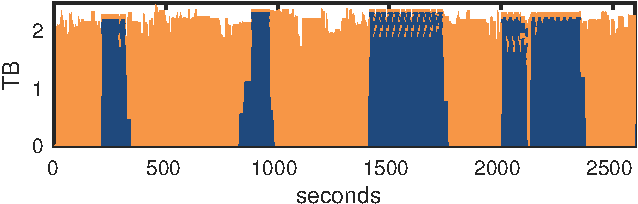
\includegraphics[width=0.8\linewidth]{fig/b1_mov_SpeedFair_BB} 
    \caption{[Cluster] \name's solution for the motivational problem (\S\ref{sec:ex}). The first two jobs of {\burstq} quickly finish and the last two jobs are prevented from using too much resource. This solution is close to the optimal one.}
    \label{fig:solution}
\end{figure}

Before diving into the details of our evaluation, recall the motivational problem from Section~\ref{sec:ex}. 
Figure~\ref{fig:solution} depicts how \name solves it in the testbed. \name enables the first two jobs of {\burstq} to quickly finish in 141 and 180 seconds.
For the two large jobs arriving at 1400 and 2000 seconds, the share is very large only in roughly 335 seconds but it is cut down to give back resource to {\batchq}.
%The large job arrives at 1400 seconds is not continuously allocated with large resources like SP.

\subsubsection{Performance guarantee}
\label{sec:performane_guarantee}

\begin{figure}[!t]
\centering
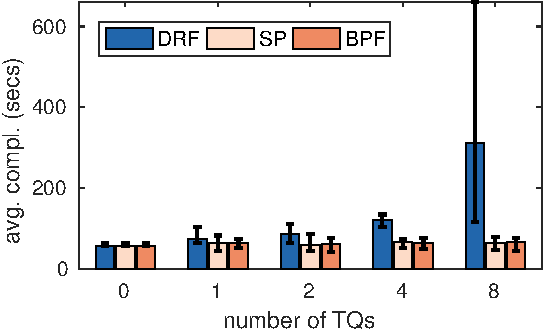
\includegraphics[width=0.8\linewidth]{fig/busty_perf_grt_err_BB}
\caption{[Cluster] Average completion time of \burstq jobs in a single \burstq across the 3 schedulers when varying the number of {\batchq}s. \name and SP guarantee the average completion time of the \burstq jobs while DRF significantly suffers from the increase of number of {\batchq}s.}
\label{fig:busty_perf_grt}
\end{figure}
 
Next, we focus on what happens when there are more than one \batchq.
Figure \ref{fig:busty_perf_grt} shows that average completion time of \burstq jobs in the 40-node cluster on the BB workload. In this setting, there are a single \burstq and multiple {\batchq}s. The x-axis shows the number of TQs in the cluster.

When there are no TQs, the average completion times of \burstq jobs across three schedulers are the same (57 seconds).
The completion times are greater than the average ON period (27 seconds) because of inefficient resource packing and allocation overheads.
In practice, the resource demand of tasks cannot utilize all resources of a node that results in large unallocated resources across multiple nodes.
Hence, the \burstq jobs are not able to receive the whole cluster capacity as expected.
More importantly, this delay is also caused by allocation overheads, such as waiting for containers to be allocated or launching containers.

As the number of {\batchq}s increases, the performance of DRF significantly degrades because DRF tends to allocate less resource to {\burstq} jobs.
DRF is the worst among three schedulers. In contrast, \name and SP give the highest priority to {\burstq}s that guarantees the performance of \burstq jobs.
The average completion times, when TQs are available (1,2,4, and 8), are almost the same (65 seconds).
These average completion times are still larger than the case of no TQs because of non-preemption.
The \burstq jobs are not able to receive the resources that are still used by the running tasks. 

\begin{table}[!t]
\centering
\caption{[Cluster] Factor of improvement by \name across various workload with respect to the number of {\batchq}s.} 
\begin{tabular}{|c|c|c|c|c|} \hline
\small
\centering
Workload & 1 TQ  & 2 TQs & 4 TQs & 8 TQs \\ \hline \hline
BB & 1.18 & 1.42 & 1.86 & 4.66 \\ \hline 
TPC-DS &  1.35 &   1.61  &  2.29  &  5.38  \\ \hline 
TPC-H & 1.10  & 1.37 & 2.01 &  5.12\\ \hline 
\end{tabular}
\label{tbl:speed_up}
\end{table}

To understand how well \name performs on various workload traces, we carried out the same experiments on TPC-DS and TPC-H.
As SP and \name achieve the similar performance, we only present the factors of improvement of \name across the various workloads in Table \ref{tbl:speed_up}.
The numbers on the table show the consistent improvement on the average completion time of \burstq jobs. 

\begin{figure}[!t]
    \centering
    \subfloat[1 LQ \& 4 TQs]{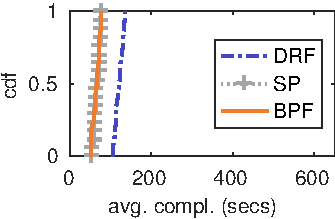
\includegraphics[width=0.48\linewidth]{fig/busty_perf_grt_cdf4_BB} \label{fig:busty_perf_grt_cdf_a}}    
    \subfloat[1 LQ \& 8 TQs]{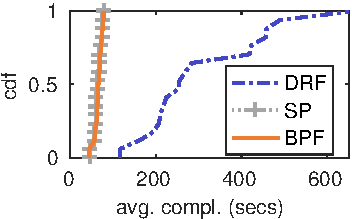
\includegraphics[width=0.48\linewidth]{fig/busty_perf_grt_cdf8_BB} \label{fig:busty_perf_grt_cdf_b}}
    \caption{[Cluster] The completion time of LQ jobs is predictable using \name.}
    \label{fig:busty_perf_grt_cdf}
    \vspace{-0.4cm}
\end{figure}

In addition to the average completion time, we evaluated the performance of individual \burstq jobs.
Figure \ref{fig:busty_perf_grt_cdf} shows that cumulative distribution functions (cdf) of the completion times across 3 approaches.
Figure \ref{fig:busty_perf_grt_cdf_a} and \ref{fig:busty_perf_grt_cdf_b} are the experimental results for the cases of 4 {\batchq}s and 8 {\batchq}s, respectively.
We observe that the completion times of \burstq jobs in DRF are not stable and vary a lot when the number of {\burstq}s becomes large as in Figure \ref{fig:busty_perf_grt_cdf_b}.
The unstable performance is caused by the instantaneous fairness and the variance of total resource demand.

\subsubsection{Fairness guarantee}
\label{sec:fairness_guarantee}

\begin{figure}[!t]
    \centering
    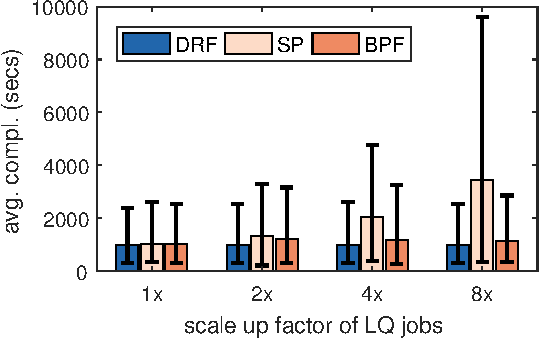
\includegraphics[width=0.8\linewidth]{fig/batch_perf_protect_BB} 
%    \\
%    \subfloat[LQ jobs]{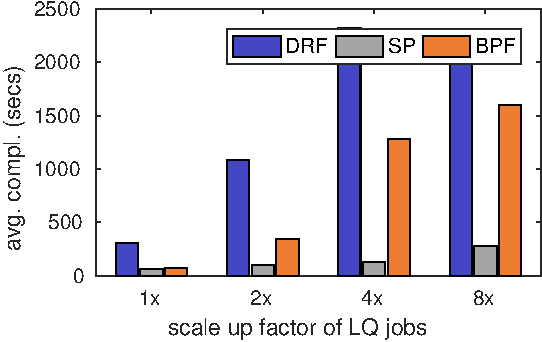
\includegraphics[width=1\linewidth]{fig/long_busty_BB} \label{fig:protecting_batch_jobs_b}}
    \caption{[Cluster] \name protects the batch jobs up to $3.05\times$ compared to SP.}
    \vspace{-0.3cm}
    \label{fig:protecting_batch_jobs}
\end{figure}

Figure \ref{fig:protecting_batch_jobs} shows the average completion time of \batchq jobs when we scale up the number of tasks of \burstq jobs are by 1x, 2x, 4x, and 8x.
In this experiment, there are a single \burstq and 8 {\batchq}s.

Since DRF is a fair scheduler, the average completion times of \batchq jobs are almost not affected by the size of \burstq jobs.
However, SP allocates too much resource to \burstq jobs that significantly hurts \batchq jobs.
Since SP provides the highest priority for the {\burstq} jobs, it makes the {\batchq} jobs to starve for resources.
\name performs closely to DRF.
While DRF maintains instantaneous fairness, \name maintains the long-term fairness among the queues.


%\begin{figure}[!t]
%\centering
%    {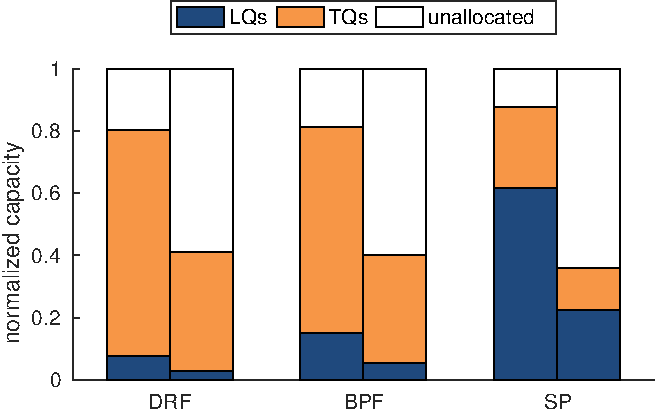
\includegraphics[width=0.8\linewidth]{fig/b8_avg_res_BB}}
%\caption{[Cluster] The average resource consumption of the cases of scaling up \burstq jobs at 8x. The left bar is memory usage, and the right bar is CPU usage. All three policies have similar utilization.}
%\label{fig:avg_res}
%\end{figure}

%To better see the long-term fairness in resource allocation, we present average resource usage across 3 approaches in Figure \ref{fig:avg_res}.
%There are totally 9 queues (1 \burstq and 8 \batchq). The x-axis is the normalized capacity.
%SP is dominant in both memory and CPU.
%\name and DRF can achieve the fairness in resource allocation for {\burstq}s and {\batchq}s.
%All of them have similar resource utilization.

\subsubsection{Scheduling overheads}

Recall from Section \ref{sec:impl} that the \name scheduler has three components: user input, admission control, and allocation.
Compared to the default schedulers in YARN, our scheduler has additional scheduling overheads for admission control and additional computation in allocation.

Since we only implement our scheduler in the Resource Manager, the scheduling overheads occur at the master node.
To measure the scheduling overheads, we run admission control for 10000 \burstq queues and 10000 \batchq queues on a master node -- Intel Xeon E3 2.4 GHz (with 12 cores).
Each LQ queue has 500 ON/OFF cycles.
Recall the \textsc{LQAdmit} and \textsc{TQAdmit} functions in Algorithm \ref{algorithm1}, the admission overheads increase linearly to the number of queues.
The total admission overheads are approximately 1 ms, which is much less than the default update interval in YARN Fair Scheduler, i.e., 500 ms \cite{hadoop-fair-scheduler}.
The additional computation in allocation is also negligibly less than 1 ms.

%\begin{table*}
%\centering
%\caption{Scheduling overheads} 
%\begin{tabular}{|c|p{10cm}|c|} \hline
%Type & Description & Avg. Time \\ \hline \hline
%Job submission & Job is submitted from client to YARN & 13.22 secs \\ \hline
%Container allocation & YARN localizes and allocates a container for a task.  &  0.04 secs \\ \hline
%Task setup & Tez setup a task to run on the allocated container. & 6.24 secs \\ \hline
%Launching Tez task & Launching a Tez task on the container & 1.17 secs \\ \hline
%Task stop & Tez stops the container use on a finished task. & 0.21 secs\\ \hline
%Container release & YARN releases the running container. & 5.19 secs \\ \hline
%\end{tabular}
%\label{tbl:schedulingOverheads}
%\end{table*}

\subsubsection{Admission control for multiple LQs}
\label{sec:admission}

\begin{figure}[!h]
	\centering
	
\includegraphics[width=0.6\linewidth]{fig/b1i3_res_usage_legend} 
	\vspace{-0.1cm}
	\subfloat[DRF: \burstq-0, \burstq-1, \burstq-2 are unhappy with high latency.]{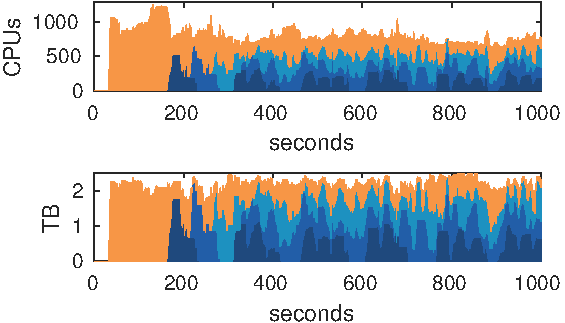
\includegraphics[width=0.8\linewidth]{fig/res_usage_b1i3_DRF_BB} \label{fig:admission_drf_cluster}} 

	\subfloat[SP: \batchq-0 is starving of resources.]{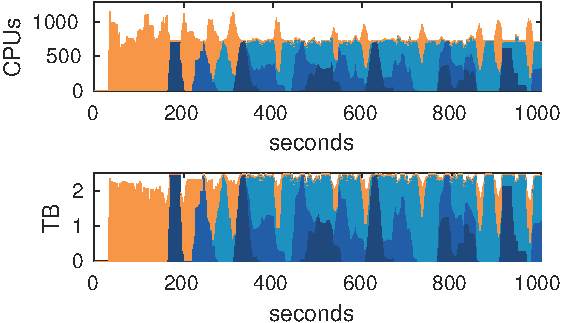
\includegraphics[width=0.8\linewidth]{fig/res_usage_b1i3_SP_BB} \label{fig:admission_strict_cluster}}
    
	\subfloat[N-\name: Only {\burstq}-0 and {\batchq}-0 are happy.]{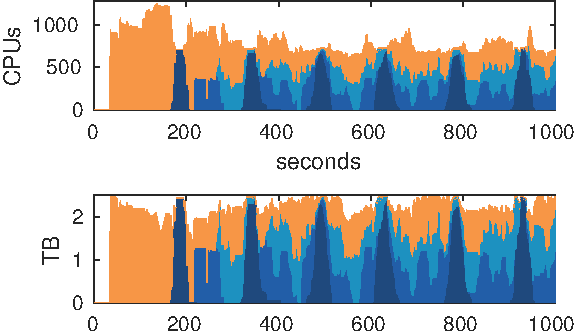
\includegraphics[width=0.8\linewidth]{fig/res_usage_b1i3_N-BPF_BB} \label{fig:admission_hard_cluster}}
   
	\subfloat[\name: {\burstq}-0, {\burstq}-1 and {\batchq}-1 are happy.]{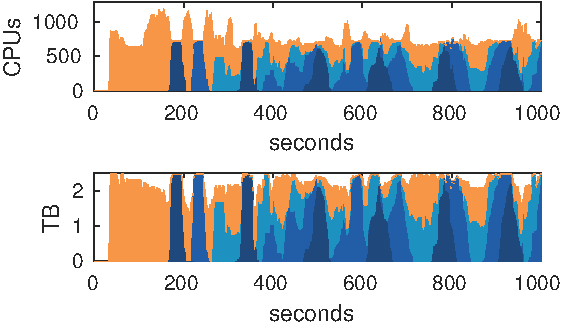
\includegraphics[width=0.8\linewidth]{fig/res_usage_b1i3_BPF_BB} \label{fig:admission_speedfair_cluster}}

	\caption{[Cluster]. DRF and SP fail to guarantee both performance and fairness simultaneously. \name gives the best performance to \burstq-0, near optimal performance for \burstq-1, and maintains fairness among 4 queues. \burstq-2 requires too much resource, so its performance cannot be guaranteed.}
	\label{fig:admission_control_cluster}
\end{figure}


To demonstrate how \name works with multiple {\burstq}s, we set up 3 {\burstq}s (\burstq-0, \burstq-1, and \burstq-2) and a single \batchq (TQ-0).
The jobs \batchq-0 are queued up at the beginning while \burstq-0, \burstq-1, and \burstq-2 arrive at 50, 100, and 150 seconds, respectively.
The periods of {\burstq}-0, {\burstq}-1, and {\burstq}-2 are 150, 110, and 60 secs. All the {\burstq}s jobs have the identical demand and task durations.
The TQ jobs are chosen from the BB benchmark.
\name admits {\burstq}-0 to the Hard Guarantee class, {\burstq}-1 to the Soft Guarantee class, and {\burstq}-2 to the Elastic class.

Figure \ref{fig:admission_drf_cluster} shows the resource usage (CPU and memory) for each queue across four schedulers, i.e., DRF, SP, N-\name and \name.
As an instantaneously fair scheduler, DRF continuously maintains the fair share for all queues as in Figure \ref{fig:admission_drf_cluster}.
Since \burstq-2 requires a lot of resources, SP makes \batchq-0 starving for resources (Figure \ref{fig:admission_strict_cluster}). N-\name provides \burstq-0 with resource guarantee and it fairly share the resources to \burstq-1, \burstq-2, and \batchq-0 (Figure \ref{fig:admission_hard_cluster}).
\name provides hard guarantee to \burstq-0 and soft guarantee to \burstq-1 as in Figure \ref{fig:admission_speedfair_cluster}.
The soft guarantee allows \burstq-1 performs better than using N-\name.
Since \burstq-2 demands too much resources, \name treats it like \batchq-0.

Figure \ref{fig:avg_multi_queue_cluster} shows the average completion time of jobs on each queue across the four schedulers.
The performance of DRF for \burstq jobs is the worst among the four schedulers but it is the best for only \batchq-0.
The performance of SP is good for \burstq jobs but it is the worst for \batchq jobs.
N-\name provides the best performance for \burstq-0 but not \burstq-1 and \burstq-2.
\name is the best among the four schedulers.
The three of four queues, i.e., \burstq-0, \burstq-1, and \batchq-0, significantly benefit from \name.
\name even outperforms SP for \burstq-0 and \burstq-1 jobs and does not hurt any {\batchq}.

\begin{figure}[!h]
	\centering
	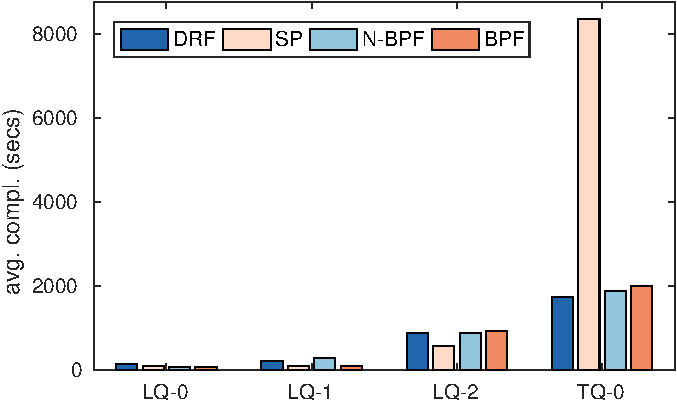
\includegraphics[width=0.8\linewidth]{fig/avg_multi_queues_impl}
	\caption{[Cluster] \name provides with better performance for {\burstq}s than DRF and N-\name. Unlike SP, \name protects the performance of \batchq jobs.}
	\label{fig:avg_multi_queue_cluster}
\end{figure}


\subsection{Performance in Trace-Driven Simulations}
\label{sec:performance_large_scale}

%\subsubsection{Benchmarks' performance in simulations}

To verify the correctness of the large-scale simulator, we replayed the BB trace logs from cluster experiments in the simulator.
Table \ref{tbl:speed_up_sim} shows the factors of improvement in completion times of \burstq jobs for BB workload in simulation that are consistent with that from our cluster experiments (Table \ref{tbl:speed_up}). 

\begin{table}[!t]
\small
\centering
\begin{tabular}{|c|c|c|c|c|c|c|} \hline
\multirow{2}{*}{Workload} &  \multicolumn{5}{c}{Number of {\batchq}s} & \\ \hhline{~------}
 & 1 & 2 & 4 & 8 & 16 & 32 \\ \hline \hline
BB & 1.08  & 1.56 & 2.32 & 4.09 & 7.28 & 16.61  \\ \hline 
TPC-DS & 1.06 & 1.38 & 1.66 & 2.93 & 5.16 & 10.40 \\ \hline 
TPC-H  & 1.01 & 1.28 & 1.92 & 3.04 & 5.50 & 11.35 \\ \hline 
\end{tabular}
\caption{[Simulation] Factors of improvement by \name across various workloads w.r.t the number of {\batchq}s.} 
\label{tbl:speed_up_sim}
\end{table}

\name significantly improves over DRF when we have more {\batchq}s.
We note that the factors of improvement for TPC-DS and TPC-H in the simulation are less that of the cluster experiments.
It turns out that DRF in TCP-DS and TPC-H suffers from the allocation overheads that our simulation does not capture.
The allocation overheads for the \burstq jobs in TPC-DS and TPC-H are large because they have more phases than the \burstq jobs in BB (only 2 phases).

%\subsubsection{Admission control for Multiple LQs}
\label{sec:admission_sim}

\begin{figure}[!h]
    \centering
    
\includegraphics[width=0.8\linewidth]{fig/res_usage_b1i3_legend} 
    \vspace{-0.2cm}
    \subfloat[DRF: \burstq-0, \burstq-1, \burstq-2 are unhappy with high latency.]{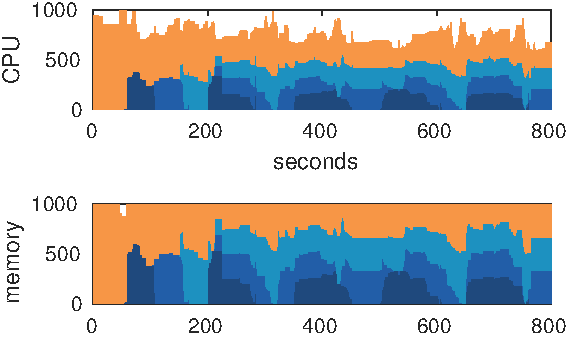
\includegraphics[width=0.8\linewidth]{fig/b1i3_res_usage_drf} \label{fig:admission_drf}} 
    \vspace{-0.1cm}
    \subfloat[SP: \batchq-0 is starving of resources.]{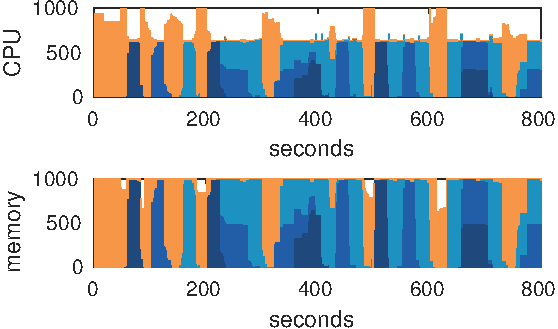
\includegraphics[width=0.8\linewidth]{fig/b1i3_res_usage_strict} \label{fig:admission_strict}}
    \vspace{-0.1cm}            
    \subfloat[N-\name: Only {\burstq}-0 and {\batchq}-0 are happy.]{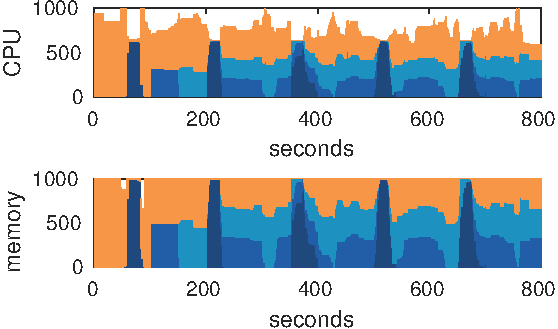
\includegraphics[width=0.8\linewidth]{fig/b1i3_res_usage_Hard} \label{fig:admission_hard}}
    \vspace{-0.1cm}    
    \subfloat[\name: {\burstq}-0, {\burstq}-1 and {\batchq}-1 are happy.]{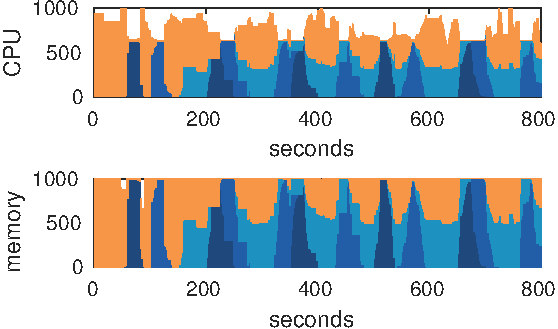
\includegraphics[width=0.8\linewidth]{fig/b1i3_res_usage_speedfair} \label{fig:admission_speedfair}}
    \vspace{-0.1cm}    
    \caption{[Simulation] DRF and SP fail to guarantee both performance and fairness simultaneously. \name gives the best performance to \burstq-0, near optimal performance for \burstq-1, and maintains fairness among 4 queues. \burstq-2 requires too much resource, so its performance cannot be guaranteed.}
    \vspace{-0.5cm}    
    \label{fig:admission_control}
\end{figure}


To demonstrate how \name works with multiple {\burstq}s, we set up 3 {\burstq}s (\burstq-0, \burstq-1, and \burstq-2) and a single \batchq (TQ-0).
The jobs \batchq-0 are queued up at the beginning while \burstq-0, \burstq-1, and \burstq-2 arrive at 50, 100, and 150 seconds, respectively.
The periods of {\burstq}-0, {\burstq}-1, and {\burstq}-2 are 150, \diff{110}, and 60 secs. All the {\burstq}s jobs have the identical demand and task durations.
The TQ jobs are chosen from the BB benchmark.
\name admits {\burstq}-0 to the Hard Guarantee class, {\burstq}-1 to the Soft Guarantee class, and {\burstq}-2 to the Elastic class.

Figure \ref{fig:admission_control} shows the resource usage (CPU and memory) for each queue across four schedulers, i.e., DRF, SP, N-\name and \name.
The capacity of CPU or memory is 1000 nodes.
As an instantaneously fair scheduler, DRF continuously maintains the fair share for all queues as in Figure \ref{fig:admission_drf}.
Since \burstq-2 requires a lot of resources, SP makes \batchq-0 starving for resources (Figure \ref{fig:admission_strict}). N-\name provides \burstq-0 with resource guarantee and it fairly share the resources to \burstq-1, \burstq-2, and \batchq-0 (Figure \ref{fig:admission_hard}).
\name provides hard guarantee to \burstq-0 and soft guarantee to \burstq-1 as in Figure \ref{fig:admission_speedfair}.
The soft guarantee allows \burstq-1 performs better than using N-\name.
Since \burstq-2 demands too much resources, \name treats it like \batchq-0.

Figure \ref{fig:avg_multi_queue} shows the average completion time of jobs on each queue across the four schedulers.
The performance of DRF for \burstq jobs is the worst among the four schedulers but it is the best for only \batchq-0.
The performance of SP is good for \burstq jobs but it is the worst for \batchq jobs.
N-\name provides the best performance for \burstq-0 but not \burstq-1 and \burstq-2.
\name is the best among the four schedulers.
The three of four queues, i.e., \burstq-0, \burstq-1, and \batchq-0, significantly benefit from \name.
\name even outperforms SP for \burstq-0 and \burstq-1 jobs and does not hurt any {\batchq}.

\begin{figure}[!h]
    \centering
    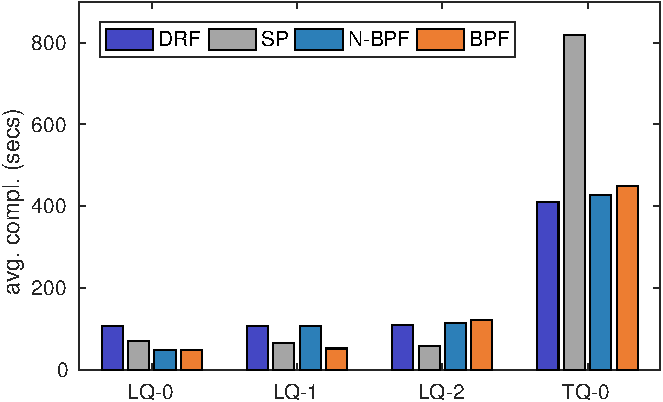
\includegraphics[width=0.8\linewidth]{fig/avg_multi_queuesadmit}
    \caption{[Simulation] \name provides with better performance for {\burstq}s than DRF and N-\name. Unlike SP, \name protects the performance of \batchq jobs.}
    \label{fig:avg_multi_queue}
\end{figure}


%\subsection{Sensitivity Analysis}
%\label{sec:sensitivity_analysis}
%
We use the large-scale simulator to study the impact of estimation errors and non-preemption on \burstq jobs. 
In both cases, \name still outperforms DRF significantly. Results are omitted due to space limit.
%
%\subsubsection{Impact of estimation errors}
%\label{sec:estimation_error_sim}
%
%\name requires users to report their estimated demand for \burstq jobs.
%However, it is challenging to estimate the demand accurately, which naturally results in estimation errors.
%To understand the impact of estimation errors on \name, we assume that estimation errors $e(\%)$ follow the standard normal distribution with zero mean.
%The standard deviation (std.) of estimation errors lines in $[0, 50]$.
%To adopt the estimation errors, we update the task demand and durations of \burstq jobs as $ {task}_{new} = {task}_{original}*(1+e/100)$.
%
%Figure \ref{fig:sen_analysis_est_err} shows the impact of estimation errors on the average completion time of \burstq jobs.
%There are 1 single \burstq and 8 {\batchq}s.
%\burstq jobs arrive every 350 seconds.
%\name is robust when the standard deviation of estimation errors vary 0 to 20.
%The \burstq jobs in BB suffer more from the large estimation errors (std. $>30$) than that of TPC-DS and TPC-H.
%The delays are caused by the underestimated jobs because the excessive demand is not guaranteed by the system.
%Meanwhile, the overestimated jobs do not suffer any delays as the guaranteed resource is more than needed.
%Although estimation errors result in performance degradation, the performance of \burstq jobs is still much better than that of DRF (162 seconds).
%%In the case of large errors, users are suggested reporting larger demands and longer stage-1 durations to improve the performance.\todo{Sentence doesn't parse.}
%
%\begin{figure}[!h]
%\centering
%    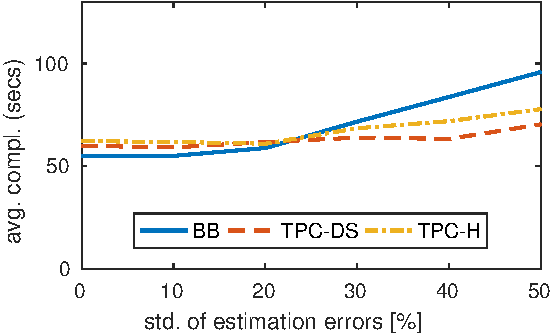
\includegraphics[width=0.7\linewidth]{fig/sen_analysis_est_err}
%\caption{[Simulation] \name's performance degrades with larger estimation errors, yet is still significantly better than DRF (162 secs).}
%\label{fig:sen_analysis_est_err}
%\end{figure}
%
%
%\subsubsection{Impact of non-preemption}
%\label{sec:non_preemption_sim}
%
%To evaluate the impact of non-preemption, we vary the average task durations of {\batchq} jobs.
%The longer task duration is, the longer the task holds its resources.
%In this evaluation, we set up 1 \burstq and 8 {\batchq}s on the simulator.
%Each \burstq job arrives every 350 secs.
%The evaluation is run on three workloads BB, TPC-DS, and TPC-H.
%
%\begin{figure}[!h]
%\centering
%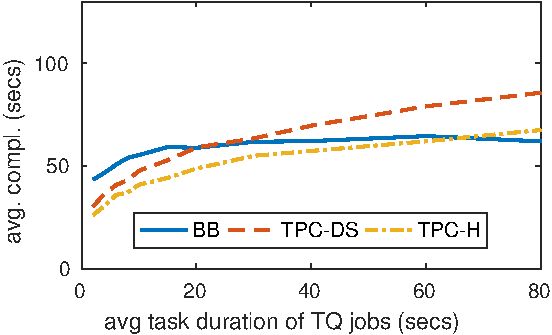
\includegraphics[width=0.7\linewidth]{fig/sen_analysis_task_duration}
%\caption{[Simulation] With longer average task durations, the impact of non-preemption on the performance of \burstq jobs becomes larger. However, the average completion time is still significantly better than that of DRF (162 secs).}
%\label{fig:sen_analysis_task_duration}
%\end{figure}
%
%Figure \ref{fig:sen_analysis_task_duration} shows the impact of average task durations of \batchq jobs on the average completion time of \burstq jobs.
%When we increase the average task durations, the performance of \burstq jobs is degraded.
%Due to the variations of task durations, the BB curve stops increasing from 20, while the TPC-DS and TPC-H curves keep going up.
%Recall the distributions of the task durations in Figure \ref{fig:worklad_cdf}: 70 percent of tasks in BB are very short.
%When the average task durations are more than 20 seconds, there are still a large number of short tasks in BB that allows \name to allocate more resources to \burstq jobs.
%TPC-DS and TPC-H have more variations of task durations that result in increasing delay for \burstq jobs.



